\documentclass[1p]{elsarticle_modified}
%\bibliographystyle{elsarticle-num}

%\usepackage[colorlinks]{hyperref}
%\usepackage{abbrmath_seonhwa} %\Abb, \Ascr, \Acal ,\Abf, \Afrak
\usepackage{amsfonts}
\usepackage{amssymb}
\usepackage{amsmath}
\usepackage{amsthm}
\usepackage{scalefnt}
\usepackage{amsbsy}
\usepackage{kotex}
\usepackage{caption}
\usepackage{subfig}
\usepackage{color}
\usepackage{graphicx}
\usepackage{xcolor} %% white, black, red, green, blue, cyan, magenta, yellow
\usepackage{float}
\usepackage{setspace}
\usepackage{hyperref}

\usepackage{tikz}
\usetikzlibrary{arrows}

\usepackage{multirow}
\usepackage{array} % fixed length table
\usepackage{hhline}

%%%%%%%%%%%%%%%%%%%%%
\makeatletter
\renewcommand*\env@matrix[1][\arraystretch]{%
	\edef\arraystretch{#1}%
	\hskip -\arraycolsep
	\let\@ifnextchar\new@ifnextchar
	\array{*\c@MaxMatrixCols c}}
\makeatother %https://tex.stackexchange.com/questions/14071/how-can-i-increase-the-line-spacing-in-a-matrix
%%%%%%%%%%%%%%%

\usepackage[normalem]{ulem}

\newcommand{\msout}[1]{\ifmmode\text{\sout{\ensuremath{#1}}}\else\sout{#1}\fi}
%SOURCE: \msout is \stkout macro in https://tex.stackexchange.com/questions/20609/strikeout-in-math-mode

\newcommand{\cancel}[1]{
	\ifmmode
	{\color{red}\msout{#1}}
	\else
	{\color{red}\sout{#1}}
	\fi
}

\newcommand{\add}[1]{
	{\color{blue}\uwave{#1}}
}

\newcommand{\replace}[2]{
	\ifmmode
	{\color{red}\msout{#1}}{\color{blue}\uwave{#2}}
	\else
	{\color{red}\sout{#1}}{\color{blue}\uwave{#2}}
	\fi
}

\newcommand{\Sol}{\mathcal{S}} %segment
\newcommand{\D}{D} %diagram
\newcommand{\A}{\mathcal{A}} %arc


%%%%%%%%%%%%%%%%%%%%%%%%%%%%%5 test

\def\sl{\operatorname{\textup{SL}}(2,\Cbb)}
\def\psl{\operatorname{\textup{PSL}}(2,\Cbb)}
\def\quan{\mkern 1mu \triangleright \mkern 1mu}

\theoremstyle{definition}
\newtheorem{thm}{Theorem}[section]
\newtheorem{prop}[thm]{Proposition}
\newtheorem{lem}[thm]{Lemma}
\newtheorem{ques}[thm]{Question}
\newtheorem{cor}[thm]{Corollary}
\newtheorem{defn}[thm]{Definition}
\newtheorem{exam}[thm]{Example}
\newtheorem{rmk}[thm]{Remark}
\newtheorem{alg}[thm]{Algorithm}

\newcommand{\I}{\sqrt{-1}}
\begin{document}

%\begin{frontmatter}
%
%\title{Boundary parabolic representations of knots up to 8 crossings}
%
%%% Group authors per affiliation:
%\author{Yunhi Cho} 
%\address{Department of Mathematics, University of Seoul, Seoul, Korea}
%\ead{yhcho@uos.ac.kr}
%
%
%\author{Seonhwa Kim} %\fnref{s_kim}}
%\address{Center for Geometry and Physics, Institute for Basic Science, Pohang, 37673, Korea}
%\ead{ryeona17@ibs.re.kr}
%
%\author{Hyuk Kim}
%\address{Department of Mathematical Sciences, Seoul National University, Seoul 08826, Korea}
%\ead{hyukkim@snu.ac.kr}
%
%\author{Seokbeom Yoon}
%\address{Department of Mathematical Sciences, Seoul National University, Seoul, 08826,  Korea}
%\ead{sbyoon15@snu.ac.kr}
%
%\begin{abstract}
%We find all boundary parabolic representation of knots up to 8 crossings.
%
%\end{abstract}
%\begin{keyword}
%    \MSC[2010] 57M25 
%\end{keyword}
%
%\end{frontmatter}

%\linenumbers
%\tableofcontents
%
\newcommand\colored[1]{\textcolor{white}{\rule[-0.35ex]{0.8em}{1.4ex}}\kern-0.8em\color{red} #1}%
%\newcommand\colored[1]{\textcolor{white}{ #1}\kern-2.17ex	\textcolor{white}{ #1}\kern-1.81ex	\textcolor{white}{ #1}\kern-2.15ex\color{red}#1	}

{\Large $\underline{12a_{1168}~(K12a_{1168})}$}

\setlength{\tabcolsep}{10pt}
\renewcommand{\arraystretch}{1.6}
\vspace{1cm}\begin{tabular}{m{100pt}>{\centering\arraybackslash}m{274pt}}
\multirow{5}{120pt}{
	\centering
	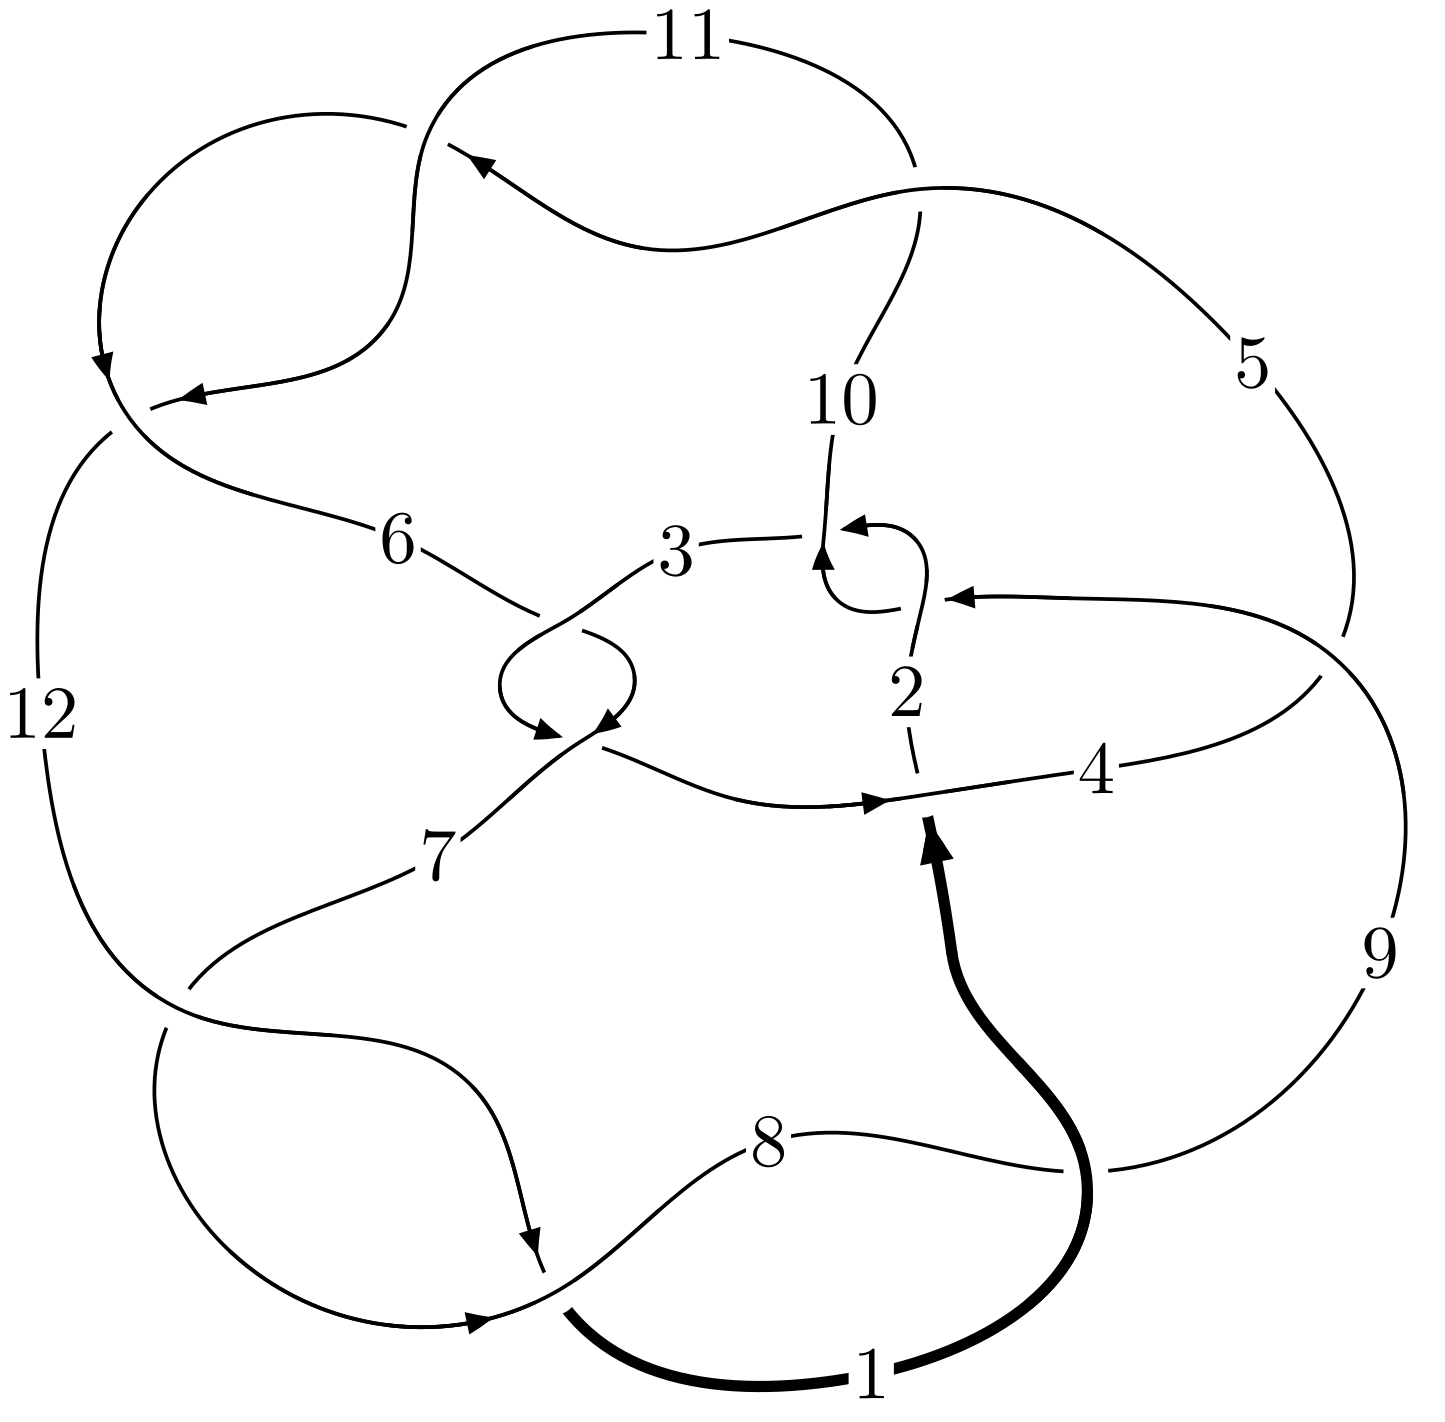
\includegraphics[width=112pt]{../../../GIT/diagram.site/Diagrams/png/1969_12a_1168.png}\\
\ \ \ A knot diagram\footnotemark}&
\allowdisplaybreaks
\textbf{Linearized knot diagam} \\
\cline{2-2}
 &
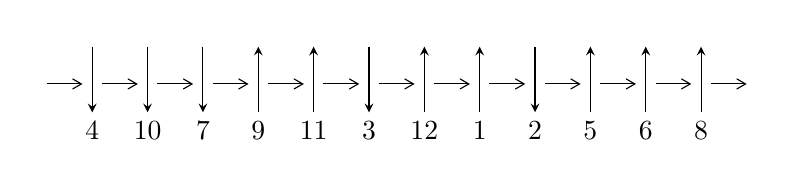
\begin{tikzpicture}[x=20pt, y=17pt]
	% nodes
	\node (C0) at (0, 0) {};
	\node (C1) at (1, 0) {};
	\node (C1U) at (1, +1) {};
	\node (C1D) at (1, -1) {4};

	\node (C2) at (2, 0) {};
	\node (C2U) at (2, +1) {};
	\node (C2D) at (2, -1) {10};

	\node (C3) at (3, 0) {};
	\node (C3U) at (3, +1) {};
	\node (C3D) at (3, -1) {7};

	\node (C4) at (4, 0) {};
	\node (C4U) at (4, +1) {};
	\node (C4D) at (4, -1) {9};

	\node (C5) at (5, 0) {};
	\node (C5U) at (5, +1) {};
	\node (C5D) at (5, -1) {11};

	\node (C6) at (6, 0) {};
	\node (C6U) at (6, +1) {};
	\node (C6D) at (6, -1) {3};

	\node (C7) at (7, 0) {};
	\node (C7U) at (7, +1) {};
	\node (C7D) at (7, -1) {12};

	\node (C8) at (8, 0) {};
	\node (C8U) at (8, +1) {};
	\node (C8D) at (8, -1) {1};

	\node (C9) at (9, 0) {};
	\node (C9U) at (9, +1) {};
	\node (C9D) at (9, -1) {2};

	\node (C10) at (10, 0) {};
	\node (C10U) at (10, +1) {};
	\node (C10D) at (10, -1) {5};

	\node (C11) at (11, 0) {};
	\node (C11U) at (11, +1) {};
	\node (C11D) at (11, -1) {6};

	\node (C12) at (12, 0) {};
	\node (C12U) at (12, +1) {};
	\node (C12D) at (12, -1) {8};
	\node (C13) at (13, 0) {};

	% arrows
	\draw[->,>={angle 60}]
	(C0) edge (C1) (C1) edge (C2) (C2) edge (C3) (C3) edge (C4) (C4) edge (C5) (C5) edge (C6) (C6) edge (C7) (C7) edge (C8) (C8) edge (C9) (C9) edge (C10) (C10) edge (C11) (C11) edge (C12) (C12) edge (C13) ;	\draw[->,>=stealth]
	(C1U) edge (C1D) (C2U) edge (C2D) (C3U) edge (C3D) (C4D) edge (C4U) (C5D) edge (C5U) (C6U) edge (C6D) (C7D) edge (C7U) (C8D) edge (C8U) (C9U) edge (C9D) (C10D) edge (C10U) (C11D) edge (C11U) (C12D) edge (C12U) ;
	\end{tikzpicture} \\
\hhline{~~} \\& 
\textbf{Solving Sequence} \\ \cline{2-2} 
 &
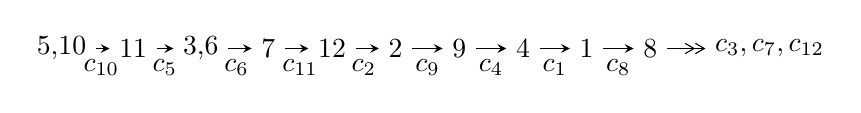
\begin{tikzpicture}[x=23pt, y=7pt]
	% node
	\node (A0) at (-1/8, 0) {5,10};
	\node (A1) at (1, 0) {11};
	\node (A2) at (33/16, 0) {3,6};
	\node (A3) at (25/8, 0) {7};
	\node (A4) at (33/8, 0) {12};
	\node (A5) at (41/8, 0) {2};
	\node (A6) at (49/8, 0) {9};
	\node (A7) at (57/8, 0) {4};
	\node (A8) at (65/8, 0) {1};
	\node (A9) at (73/8, 0) {8};
	\node (C1) at (1/2, -1) {$c_{10}$};
	\node (C2) at (3/2, -1) {$c_{5}$};
	\node (C3) at (21/8, -1) {$c_{6}$};
	\node (C4) at (29/8, -1) {$c_{11}$};
	\node (C5) at (37/8, -1) {$c_{2}$};
	\node (C6) at (45/8, -1) {$c_{9}$};
	\node (C7) at (53/8, -1) {$c_{4}$};
	\node (C8) at (61/8, -1) {$c_{1}$};
	\node (C9) at (69/8, -1) {$c_{8}$};
	\node (A10) at (11, 0) {$c_{3},c_{7},c_{12}$};

	% edge
	\draw[->,>=stealth]	
	(A0) edge (A1) (A1) edge (A2) (A2) edge (A3) (A3) edge (A4) (A4) edge (A5) (A5) edge (A6) (A6) edge (A7) (A7) edge (A8) (A8) edge (A9) ;
	\draw[->>,>={angle 60}]	
	(A9) edge (A10);
\end{tikzpicture} \\ 

\end{tabular} \\

\footnotetext{
The image of knot diagram is generated by the software ``\textbf{Draw programme}" developed by Andrew Bartholomew(\url{http://www.layer8.co.uk/maths/draw/index.htm\#Running-draw}), where we modified some parts for our purpose(\url{https://github.com/CATsTAILs/LinksPainter}).
}\phantom \\ \newline 
\centering \textbf{Ideals for irreducible components\footnotemark of $X_{\text{par}}$} 
 
\begin{align*}
I^u_{1}&=\langle 
-1.02112\times10^{219} u^{97}+2.42861\times10^{219} u^{96}+\cdots+1.88853\times10^{219} b+4.15398\times10^{220},\\
\phantom{I^u_{1}}&\phantom{= \langle  }7.40552\times10^{221} u^{97}-1.66364\times10^{222} u^{96}+\cdots+8.12069\times10^{220} a-2.62723\times10^{223},\\
\phantom{I^u_{1}}&\phantom{= \langle  }u^{98}- u^{97}+\cdots+396 u-43\rangle \\
I^u_{2}&=\langle 
-18 u^{20}+35 u^{19}+\cdots+31 b+81,\;-29 u^{20}+3 u^{19}+\cdots+31 a+84,\;u^{21}-12 u^{19}+\cdots- u-1\rangle \\
\\
\end{align*}
\raggedright * 2 irreducible components of $\dim_{\mathbb{C}}=0$, with total 119 representations.\\
\footnotetext{All coefficients of polynomials are rational numbers. But the coefficients are sometimes approximated in decimal forms when there is not enough margin.}
\newpage
\renewcommand{\arraystretch}{1}
\centering \section*{I. $I^u_{1}= \langle -1.02\times10^{219} u^{97}+2.43\times10^{219} u^{96}+\cdots+1.89\times10^{219} b+4.15\times10^{220},\;7.41\times10^{221} u^{97}-1.66\times10^{222} u^{96}+\cdots+8.12\times10^{220} a-2.63\times10^{223},\;u^{98}- u^{97}+\cdots+396 u-43 \rangle$}
\flushleft \textbf{(i) Arc colorings}\\
\begin{tabular}{m{7pt} m{180pt} m{7pt} m{180pt} }
\flushright $a_{5}=$&$\begin{pmatrix}0\\u\end{pmatrix}$ \\
\flushright $a_{10}=$&$\begin{pmatrix}1\\0\end{pmatrix}$ \\
\flushright $a_{11}=$&$\begin{pmatrix}1\\- u^2\end{pmatrix}$ \\
\flushright $a_{3}=$&$\begin{pmatrix}-9.11932 u^{97}+20.4864 u^{96}+\cdots-3188.58 u+323.523\\0.540697 u^{97}-1.28598 u^{96}+\cdots+214.779 u-21.9958\end{pmatrix}$ \\
\flushright $a_{6}=$&$\begin{pmatrix}u\\- u^3+u\end{pmatrix}$ \\
\flushright $a_{7}=$&$\begin{pmatrix}-8.60049 u^{97}+19.0570 u^{96}+\cdots-2814.24 u+268.683\\-3.34750 u^{97}+7.42210 u^{96}+\cdots-1148.85 u+116.947\end{pmatrix}$ \\
\flushright $a_{12}=$&$\begin{pmatrix}- u^2+1\\u^4-2 u^2\end{pmatrix}$ \\
\flushright $a_{2}=$&$\begin{pmatrix}-8.57862 u^{97}+19.2004 u^{96}+\cdots-2973.80 u+301.528\\0.540697 u^{97}-1.28598 u^{96}+\cdots+214.779 u-21.9958\end{pmatrix}$ \\
\flushright $a_{9}=$&$\begin{pmatrix}-6.09442 u^{97}+13.8926 u^{96}+\cdots-2230.11 u+230.240\\1.83837 u^{97}-4.17749 u^{96}+\cdots+651.713 u-66.9090\end{pmatrix}$ \\
\flushright $a_{4}=$&$\begin{pmatrix}-2.31310 u^{97}+5.17198 u^{96}+\cdots-655.200 u+50.8427\\5.33139 u^{97}-11.6945 u^{96}+\cdots+1763.76 u-172.869\end{pmatrix}$ \\
\flushright $a_{1}=$&$\begin{pmatrix}-1.29885 u^{97}+2.94361 u^{96}+\cdots-318.314 u+17.2269\\1.39998 u^{97}-3.01976 u^{96}+\cdots+427.622 u-39.1893\end{pmatrix}$ \\
\flushright $a_{8}=$&$\begin{pmatrix}-6.34467 u^{97}+13.9931 u^{96}+\cdots-2044.24 u+193.324\\-0.534636 u^{97}+1.09416 u^{96}+\cdots-173.613 u+19.4352\end{pmatrix}$\\&\end{tabular}
\flushleft \textbf{(ii) Obstruction class $= -1$}\\~\\
\flushleft \textbf{(iii) Cusp Shapes $= 19.4904 u^{97}-44.0633 u^{96}+\cdots+7002.50 u-705.505$}\\~\\
\newpage\renewcommand{\arraystretch}{1}
\flushleft \textbf{(iv) u-Polynomials at the component}\newline \\
\begin{tabular}{m{50pt}|m{274pt}}
Crossings & \hspace{64pt}u-Polynomials at each crossing \\
\hline $$\begin{aligned}c_{1}\end{aligned}$$&$\begin{aligned}
&u^{98}- u^{97}+\cdots+5 u-1
\end{aligned}$\\
\hline $$\begin{aligned}c_{2},c_{9}\end{aligned}$$&$\begin{aligned}
&u^{98}-33 u^{96}+\cdots-1246 u-76
\end{aligned}$\\
\hline $$\begin{aligned}c_{3},c_{6}\end{aligned}$$&$\begin{aligned}
&u^{98}-2 u^{97}+\cdots-6 u+1
\end{aligned}$\\
\hline $$\begin{aligned}c_{4}\end{aligned}$$&$\begin{aligned}
&u^{98}+3 u^{97}+\cdots-1183 u-187
\end{aligned}$\\
\hline $$\begin{aligned}c_{5},c_{10},c_{11}\end{aligned}$$&$\begin{aligned}
&u^{98}- u^{97}+\cdots+396 u-43
\end{aligned}$\\
\hline $$\begin{aligned}c_{7},c_{8},c_{12}\end{aligned}$$&$\begin{aligned}
&u^{98}+3 u^{97}+\cdots+32 u+1
\end{aligned}$\\
\hline
\end{tabular}\\~\\
\newpage\renewcommand{\arraystretch}{1}
\flushleft \textbf{(v) Riley Polynomials at the component}\newline \\
\begin{tabular}{m{50pt}|m{274pt}}
Crossings & \hspace{64pt}Riley Polynomials at each crossing \\
\hline $$\begin{aligned}c_{1}\end{aligned}$$&$\begin{aligned}
&y^{98}-3 y^{97}+\cdots+173 y+1
\end{aligned}$\\
\hline $$\begin{aligned}c_{2},c_{9}\end{aligned}$$&$\begin{aligned}
&y^{98}-66 y^{97}+\cdots-1035260 y+5776
\end{aligned}$\\
\hline $$\begin{aligned}c_{3},c_{6}\end{aligned}$$&$\begin{aligned}
&y^{98}-54 y^{97}+\cdots+132 y+1
\end{aligned}$\\
\hline $$\begin{aligned}c_{4}\end{aligned}$$&$\begin{aligned}
&y^{98}-25 y^{97}+\cdots-1527771 y+34969
\end{aligned}$\\
\hline $$\begin{aligned}c_{5},c_{10},c_{11}\end{aligned}$$&$\begin{aligned}
&y^{98}-97 y^{97}+\cdots+29288 y+1849
\end{aligned}$\\
\hline $$\begin{aligned}c_{7},c_{8},c_{12}\end{aligned}$$&$\begin{aligned}
&y^{98}-105 y^{97}+\cdots-568 y+1
\end{aligned}$\\
\hline
\end{tabular}\\~\\
\newpage\flushleft \textbf{(vi) Complex Volumes and Cusp Shapes}
$$\begin{array}{c|c|c}  
\text{Solutions to }I^u_{1}& \I (\text{vol} + \sqrt{-1}CS) & \text{Cusp shape}\\
 \hline 
\begin{aligned}
u &= \phantom{-}0.438752 + 0.891193 I \\
a &= \phantom{-}0.362502 + 0.686195 I \\
b &= \phantom{-}1.303190 - 0.450763 I\end{aligned}
 & -5.41570 + 8.09818 I & \phantom{-0.000000 } 0 \\ \hline\begin{aligned}
u &= \phantom{-}0.438752 - 0.891193 I \\
a &= \phantom{-}0.362502 - 0.686195 I \\
b &= \phantom{-}1.303190 + 0.450763 I\end{aligned}
 & -5.41570 - 8.09818 I & \phantom{-0.000000 } 0 \\ \hline\begin{aligned}
u &= \phantom{-}0.391864 + 0.898326 I \\
a &= \phantom{-}0.903543 - 0.068277 I \\
b &= \phantom{-}0.528510 - 0.233621 I\end{aligned}
 & \phantom{-}4.41768 - 2.63930 I & \phantom{-0.000000 } 0 \\ \hline\begin{aligned}
u &= \phantom{-}0.391864 - 0.898326 I \\
a &= \phantom{-}0.903543 + 0.068277 I \\
b &= \phantom{-}0.528510 + 0.233621 I\end{aligned}
 & \phantom{-}4.41768 + 2.63930 I & \phantom{-0.000000 } 0 \\ \hline\begin{aligned}
u &= \phantom{-}0.391411 + 0.898450 I \\
a &= \phantom{-}0.580518 - 0.049871 I \\
b &= \phantom{-}0.939209 + 0.499556 I\end{aligned}
 & \phantom{-}2.92084 - 1.91064 I & \phantom{-0.000000 } 0 \\ \hline\begin{aligned}
u &= \phantom{-}0.391411 - 0.898450 I \\
a &= \phantom{-}0.580518 + 0.049871 I \\
b &= \phantom{-}0.939209 - 0.499556 I\end{aligned}
 & \phantom{-}2.92084 + 1.91064 I & \phantom{-0.000000 } 0 \\ \hline\begin{aligned}
u &= \phantom{-}0.938750 + 0.254685 I \\
a &= \phantom{-}0.112409 + 0.225776 I \\
b &= \phantom{-}1.381750 - 0.029759 I\end{aligned}
 & \phantom{-}1.79041 - 0.16871 I & \phantom{-0.000000 } 0 \\ \hline\begin{aligned}
u &= \phantom{-}0.938750 - 0.254685 I \\
a &= \phantom{-}0.112409 - 0.225776 I \\
b &= \phantom{-}1.381750 + 0.029759 I\end{aligned}
 & \phantom{-}1.79041 + 0.16871 I & \phantom{-0.000000 } 0 \\ \hline\begin{aligned}
u &= -0.852144 + 0.390335 I \\
a &= \phantom{-}0.578814 - 0.432802 I \\
b &= -0.246807 + 0.692959 I\end{aligned}
 & \phantom{-}6.86100 - 2.05030 I & \phantom{-0.000000 } 0 \\ \hline\begin{aligned}
u &= -0.852144 - 0.390335 I \\
a &= \phantom{-}0.578814 + 0.432802 I \\
b &= -0.246807 - 0.692959 I\end{aligned}
 & \phantom{-}6.86100 + 2.05030 I & \phantom{-0.000000 } 0\\
 \hline 
 \end{array}$$\newpage$$\begin{array}{c|c|c}  
\text{Solutions to }I^u_{1}& \I (\text{vol} + \sqrt{-1}CS) & \text{Cusp shape}\\
 \hline 
\begin{aligned}
u &= -0.915479\phantom{ +0.000000I} \\
a &= -1.31935\phantom{ +0.000000I} \\
b &= \phantom{-}1.49906\phantom{ +0.000000I}\end{aligned}
 & -5.21283\phantom{ +0.000000I} & \phantom{-0.000000 } 0 \\ \hline\begin{aligned}
u &= -0.058479 + 0.894470 I \\
a &= \phantom{-}0.577736 - 0.337542 I \\
b &= \phantom{-}0.458079 + 0.502884 I\end{aligned}
 & \phantom{-}4.16131 - 2.22766 I & \phantom{-0.000000 } 0 \\ \hline\begin{aligned}
u &= -0.058479 - 0.894470 I \\
a &= \phantom{-}0.577736 + 0.337542 I \\
b &= \phantom{-}0.458079 - 0.502884 I\end{aligned}
 & \phantom{-}4.16131 + 2.22766 I & \phantom{-0.000000 } 0 \\ \hline\begin{aligned}
u &= -0.446241 + 1.029130 I \\
a &= -0.434185 + 0.599991 I \\
b &= -1.262990 - 0.482764 I\end{aligned}
 & \phantom{-}1.37895 - 11.98030 I & \phantom{-0.000000 } 0 \\ \hline\begin{aligned}
u &= -0.446241 - 1.029130 I \\
a &= -0.434185 - 0.599991 I \\
b &= -1.262990 + 0.482764 I\end{aligned}
 & \phantom{-}1.37895 + 11.98030 I & \phantom{-0.000000 } 0 \\ \hline\begin{aligned}
u &= \phantom{-}0.792923 + 0.793440 I \\
a &= \phantom{-}0.282718 - 0.510672 I \\
b &= -1.156990 - 0.219396 I\end{aligned}
 & -4.42238 - 2.43268 I & \phantom{-0.000000 } 0 \\ \hline\begin{aligned}
u &= \phantom{-}0.792923 - 0.793440 I \\
a &= \phantom{-}0.282718 + 0.510672 I \\
b &= -1.156990 + 0.219396 I\end{aligned}
 & -4.42238 + 2.43268 I & \phantom{-0.000000 } 0 \\ \hline\begin{aligned}
u &= \phantom{-}1.132050 + 0.247239 I \\
a &= -0.15095 - 2.01792 I \\
b &= -1.047450 + 0.584414 I\end{aligned}
 & \phantom{-}4.99022 + 6.27593 I & \phantom{-0.000000 } 0 \\ \hline\begin{aligned}
u &= \phantom{-}1.132050 - 0.247239 I \\
a &= -0.15095 + 2.01792 I \\
b &= -1.047450 - 0.584414 I\end{aligned}
 & \phantom{-}4.99022 - 6.27593 I & \phantom{-0.000000 } 0 \\ \hline\begin{aligned}
u &= -0.456258 + 0.670176 I \\
a &= -0.171983 + 0.785584 I \\
b &= -1.36966 - 0.40803 I\end{aligned}
 & -5.36300 - 2.92221 I & \phantom{-0.000000 } 0\\
 \hline 
 \end{array}$$\newpage$$\begin{array}{c|c|c}  
\text{Solutions to }I^u_{1}& \I (\text{vol} + \sqrt{-1}CS) & \text{Cusp shape}\\
 \hline 
\begin{aligned}
u &= -0.456258 - 0.670176 I \\
a &= -0.171983 - 0.785584 I \\
b &= -1.36966 + 0.40803 I\end{aligned}
 & -5.36300 + 2.92221 I & \phantom{-0.000000 } 0 \\ \hline\begin{aligned}
u &= -0.106869 + 0.787117 I \\
a &= -0.807532 - 0.213605 I \\
b &= -0.822220 + 0.300167 I\end{aligned}
 & -1.42261 + 1.54220 I & \phantom{-0.000000 } 0 \\ \hline\begin{aligned}
u &= -0.106869 - 0.787117 I \\
a &= -0.807532 + 0.213605 I \\
b &= -0.822220 - 0.300167 I\end{aligned}
 & -1.42261 - 1.54220 I & \phantom{-0.000000 } 0 \\ \hline\begin{aligned}
u &= \phantom{-}0.513550 + 0.603793 I \\
a &= -0.410518 + 0.368788 I \\
b &= \phantom{-}0.041349 - 0.849349 I\end{aligned}
 & \phantom{-}5.22586 + 7.17879 I & \phantom{-0.000000 } 0 \\ \hline\begin{aligned}
u &= \phantom{-}0.513550 - 0.603793 I \\
a &= -0.410518 - 0.368788 I \\
b &= \phantom{-}0.041349 + 0.849349 I\end{aligned}
 & \phantom{-}5.22586 - 7.17879 I & \phantom{-0.000000 } 0 \\ \hline\begin{aligned}
u &= \phantom{-}1.210380 + 0.055278 I \\
a &= -0.64806 - 1.90999 I \\
b &= \phantom{-}0.729911 + 0.089716 I\end{aligned}
 & \phantom{-}6.09977 + 5.59032 I & \phantom{-0.000000 } 0 \\ \hline\begin{aligned}
u &= \phantom{-}1.210380 - 0.055278 I \\
a &= -0.64806 + 1.90999 I \\
b &= \phantom{-}0.729911 - 0.089716 I\end{aligned}
 & \phantom{-}6.09977 - 5.59032 I & \phantom{-0.000000 } 0 \\ \hline\begin{aligned}
u &= -1.22310\phantom{ +0.000000I} \\
a &= -0.188603\phantom{ +0.000000I} \\
b &= -1.50392\phantom{ +0.000000I}\end{aligned}
 & -3.65106\phantom{ +0.000000I} & \phantom{-0.000000 } 0 \\ \hline\begin{aligned}
u &= \phantom{-}0.774695\phantom{ +0.000000I} \\
a &= \phantom{-}0.494111\phantom{ +0.000000I} \\
b &= \phantom{-}0.985875\phantom{ +0.000000I}\end{aligned}
 & \phantom{-}2.30370\phantom{ +0.000000I} & \phantom{-}4.50380\phantom{ +0.000000I} \\ \hline\begin{aligned}
u &= -1.245610 + 0.001635 I \\
a &= \phantom{-}0.11423 + 1.54880 I \\
b &= -0.806424 - 0.186193 I\end{aligned}
 & \phantom{-}1.05719 + 2.40310 I & \phantom{-0.000000 } 0\\
 \hline 
 \end{array}$$\newpage$$\begin{array}{c|c|c}  
\text{Solutions to }I^u_{1}& \I (\text{vol} + \sqrt{-1}CS) & \text{Cusp shape}\\
 \hline 
\begin{aligned}
u &= -1.245610 - 0.001635 I \\
a &= \phantom{-}0.11423 - 1.54880 I \\
b &= -0.806424 + 0.186193 I\end{aligned}
 & \phantom{-}1.05719 - 2.40310 I & \phantom{-0.000000 } 0 \\ \hline\begin{aligned}
u &= -0.397002 + 0.606555 I \\
a &= -0.06672 - 1.47204 I \\
b &= \phantom{-}1.206540 - 0.037207 I\end{aligned}
 & -5.34711 - 1.16504 I & -5.89004 + 4.77110 I \\ \hline\begin{aligned}
u &= -0.397002 - 0.606555 I \\
a &= -0.06672 + 1.47204 I \\
b &= \phantom{-}1.206540 + 0.037207 I\end{aligned}
 & -5.34711 + 1.16504 I & -5.89004 - 4.77110 I \\ \hline\begin{aligned}
u &= \phantom{-}0.197358 + 0.695563 I \\
a &= -1.05863 - 1.44758 I \\
b &= -1.209490 + 0.094174 I\end{aligned}
 & -0.50881 + 3.77042 I & -1.22991 - 5.05475 I \\ \hline\begin{aligned}
u &= \phantom{-}0.197358 - 0.695563 I \\
a &= -1.05863 + 1.44758 I \\
b &= -1.209490 - 0.094174 I\end{aligned}
 & -0.50881 - 3.77042 I & -1.22991 + 5.05475 I \\ \hline\begin{aligned}
u &= -1.289390 + 0.036606 I \\
a &= -0.57450 - 1.79709 I \\
b &= \phantom{-}1.16868 + 0.84371 I\end{aligned}
 & \phantom{-}1.64723 - 2.83590 I & \phantom{-0.000000 } 0 \\ \hline\begin{aligned}
u &= -1.289390 - 0.036606 I \\
a &= -0.57450 + 1.79709 I \\
b &= \phantom{-}1.16868 - 0.84371 I\end{aligned}
 & \phantom{-}1.64723 + 2.83590 I & \phantom{-0.000000 } 0 \\ \hline\begin{aligned}
u &= \phantom{-}1.322300 + 0.134120 I \\
a &= \phantom{-}0.037004 + 1.012680 I \\
b &= \phantom{-}0.967591 - 0.296262 I\end{aligned}
 & \phantom{-}2.99763 + 1.06282 I & \phantom{-0.000000 } 0 \\ \hline\begin{aligned}
u &= \phantom{-}1.322300 - 0.134120 I \\
a &= \phantom{-}0.037004 - 1.012680 I \\
b &= \phantom{-}0.967591 + 0.296262 I\end{aligned}
 & \phantom{-}2.99763 - 1.06282 I & \phantom{-0.000000 } 0 \\ \hline\begin{aligned}
u &= -1.329790 + 0.051565 I \\
a &= \phantom{-}0.714474 - 1.092350 I \\
b &= -0.429983 + 0.762264 I\end{aligned}
 & \phantom{-}6.66431 - 1.15467 I & \phantom{-0.000000 } 0\\
 \hline 
 \end{array}$$\newpage$$\begin{array}{c|c|c}  
\text{Solutions to }I^u_{1}& \I (\text{vol} + \sqrt{-1}CS) & \text{Cusp shape}\\
 \hline 
\begin{aligned}
u &= -1.329790 - 0.051565 I \\
a &= \phantom{-}0.714474 + 1.092350 I \\
b &= -0.429983 - 0.762264 I\end{aligned}
 & \phantom{-}6.66431 + 1.15467 I & \phantom{-0.000000 } 0 \\ \hline\begin{aligned}
u &= \phantom{-}0.474672 + 0.455473 I \\
a &= -1.79909 - 1.37357 I \\
b &= -1.117410 + 0.415698 I\end{aligned}
 & \phantom{-}4.31172 + 6.23668 I & \phantom{-}4.72015 - 6.34301 I \\ \hline\begin{aligned}
u &= \phantom{-}0.474672 - 0.455473 I \\
a &= -1.79909 + 1.37357 I \\
b &= -1.117410 - 0.415698 I\end{aligned}
 & \phantom{-}4.31172 - 6.23668 I & \phantom{-}4.72015 + 6.34301 I \\ \hline\begin{aligned}
u &= \phantom{-}1.34546\phantom{ +0.000000I} \\
a &= \phantom{-}0.218883\phantom{ +0.000000I} \\
b &= \phantom{-}1.55069\phantom{ +0.000000I}\end{aligned}
 & \phantom{-}1.09642\phantom{ +0.000000I} & \phantom{-0.000000 } 0 \\ \hline\begin{aligned}
u &= \phantom{-}1.370950 + 0.051265 I \\
a &= \phantom{-}1.02671 + 1.27373 I \\
b &= -1.64996 - 0.89336 I\end{aligned}
 & \phantom{-}6.60733 + 2.66078 I & \phantom{-0.000000 } 0 \\ \hline\begin{aligned}
u &= \phantom{-}1.370950 - 0.051265 I \\
a &= \phantom{-}1.02671 - 1.27373 I \\
b &= -1.64996 + 0.89336 I\end{aligned}
 & \phantom{-}6.60733 - 2.66078 I & \phantom{-0.000000 } 0 \\ \hline\begin{aligned}
u &= \phantom{-}1.384850 + 0.203389 I \\
a &= \phantom{-}0.14247 - 1.56229 I \\
b &= -1.252250 + 0.535982 I\end{aligned}
 & \phantom{-}3.79747 + 6.54307 I & \phantom{-0.000000 } 0 \\ \hline\begin{aligned}
u &= \phantom{-}1.384850 - 0.203389 I \\
a &= \phantom{-}0.14247 + 1.56229 I \\
b &= -1.252250 - 0.535982 I\end{aligned}
 & \phantom{-}3.79747 - 6.54307 I & \phantom{-0.000000 } 0 \\ \hline\begin{aligned}
u &= -1.378540 + 0.268996 I \\
a &= -0.36382 - 1.84575 I \\
b &= \phantom{-}1.103300 + 0.247597 I\end{aligned}
 & \phantom{-}4.49819 - 7.25601 I & \phantom{-0.000000 } 0 \\ \hline\begin{aligned}
u &= -1.378540 - 0.268996 I \\
a &= -0.36382 + 1.84575 I \\
b &= \phantom{-}1.103300 - 0.247597 I\end{aligned}
 & \phantom{-}4.49819 + 7.25601 I & \phantom{-0.000000 } 0\\
 \hline 
 \end{array}$$\newpage$$\begin{array}{c|c|c}  
\text{Solutions to }I^u_{1}& \I (\text{vol} + \sqrt{-1}CS) & \text{Cusp shape}\\
 \hline 
\begin{aligned}
u &= -0.996538 + 0.995942 I \\
a &= -0.147207 - 0.267647 I \\
b &= \phantom{-}1.054030 - 0.308627 I\end{aligned}
 & \phantom{-}2.76808 + 5.25836 I & \phantom{-0.000000 } 0 \\ \hline\begin{aligned}
u &= -0.996538 - 0.995942 I \\
a &= -0.147207 + 0.267647 I \\
b &= \phantom{-}1.054030 + 0.308627 I\end{aligned}
 & \phantom{-}2.76808 - 5.25836 I & \phantom{-0.000000 } 0 \\ \hline\begin{aligned}
u &= -1.412160 + 0.029118 I \\
a &= \phantom{-}0.57366 + 1.41669 I \\
b &= -0.398717 - 1.040950 I\end{aligned}
 & \phantom{-}6.77476 + 1.07902 I & \phantom{-0.000000 } 0 \\ \hline\begin{aligned}
u &= -1.412160 - 0.029118 I \\
a &= \phantom{-}0.57366 - 1.41669 I \\
b &= -0.398717 + 1.040950 I\end{aligned}
 & \phantom{-}6.77476 - 1.07902 I & \phantom{-0.000000 } 0 \\ \hline\begin{aligned}
u &= \phantom{-}1.40716 + 0.19956 I \\
a &= -0.442205 - 0.849721 I \\
b &= \phantom{-}0.591377 + 0.673716 I\end{aligned}
 & \phantom{-}3.94160 + 1.46877 I & \phantom{-0.000000 } 0 \\ \hline\begin{aligned}
u &= \phantom{-}1.40716 - 0.19956 I \\
a &= -0.442205 + 0.849721 I \\
b &= \phantom{-}0.591377 - 0.673716 I\end{aligned}
 & \phantom{-}3.94160 - 1.46877 I & \phantom{-0.000000 } 0 \\ \hline\begin{aligned}
u &= -0.251196 + 0.515381 I \\
a &= \phantom{-}1.77432 - 0.77605 I \\
b &= \phantom{-}1.081420 + 0.350458 I\end{aligned}
 & -1.42079 - 3.86409 I & \phantom{-}0.73110 + 8.65417 I \\ \hline\begin{aligned}
u &= -0.251196 - 0.515381 I \\
a &= \phantom{-}1.77432 + 0.77605 I \\
b &= \phantom{-}1.081420 - 0.350458 I\end{aligned}
 & -1.42079 + 3.86409 I & \phantom{-}0.73110 - 8.65417 I \\ \hline\begin{aligned}
u &= -1.37807 + 0.38773 I \\
a &= \phantom{-}0.048832 - 1.378100 I \\
b &= \phantom{-}0.969732 + 0.514999 I\end{aligned}
 & \phantom{-}2.80879 - 6.07718 I & \phantom{-0.000000 } 0 \\ \hline\begin{aligned}
u &= -1.37807 - 0.38773 I \\
a &= \phantom{-}0.048832 + 1.378100 I \\
b &= \phantom{-}0.969732 - 0.514999 I\end{aligned}
 & \phantom{-}2.80879 + 6.07718 I & \phantom{-0.000000 } 0\\
 \hline 
 \end{array}$$\newpage$$\begin{array}{c|c|c}  
\text{Solutions to }I^u_{1}& \I (\text{vol} + \sqrt{-1}CS) & \text{Cusp shape}\\
 \hline 
\begin{aligned}
u &= -0.192714 + 0.527897 I \\
a &= -0.968831 + 0.219684 I \\
b &= -0.933289 + 0.345314 I\end{aligned}
 & -1.44128 + 1.38418 I & \phantom{-}1.09886 + 2.24692 I \\ \hline\begin{aligned}
u &= -0.192714 - 0.527897 I \\
a &= -0.968831 - 0.219684 I \\
b &= -0.933289 - 0.345314 I\end{aligned}
 & -1.44128 - 1.38418 I & \phantom{-}1.09886 - 2.24692 I \\ \hline\begin{aligned}
u &= \phantom{-}1.43811 + 0.15125 I \\
a &= \phantom{-}0.11771 + 1.79107 I \\
b &= -0.04379 - 1.48336 I\end{aligned}
 & \phantom{-}4.84521 + 5.36107 I & \phantom{-0.000000 } 0 \\ \hline\begin{aligned}
u &= \phantom{-}1.43811 - 0.15125 I \\
a &= \phantom{-}0.11771 - 1.79107 I \\
b &= -0.04379 + 1.48336 I\end{aligned}
 & \phantom{-}4.84521 - 5.36107 I & \phantom{-0.000000 } 0 \\ \hline\begin{aligned}
u &= \phantom{-}1.43863 + 0.23949 I \\
a &= \phantom{-}0.69528 - 1.36386 I \\
b &= -0.966754 + 0.214159 I\end{aligned}
 & \phantom{-}0.49710 + 4.31155 I & \phantom{-0.000000 } 0 \\ \hline\begin{aligned}
u &= \phantom{-}1.43863 - 0.23949 I \\
a &= \phantom{-}0.69528 + 1.36386 I \\
b &= -0.966754 - 0.214159 I\end{aligned}
 & \phantom{-}0.49710 - 4.31155 I & \phantom{-0.000000 } 0 \\ \hline\begin{aligned}
u &= \phantom{-}0.537595\phantom{ +0.000000I} \\
a &= \phantom{-}3.07677\phantom{ +0.000000I} \\
b &= -0.133007\phantom{ +0.000000I}\end{aligned}
 & \phantom{-}1.02611\phantom{ +0.000000I} & \phantom{-}14.3890\phantom{ +0.000000I} \\ \hline\begin{aligned}
u &= -0.212695 + 0.474080 I \\
a &= -1.25749 - 0.94890 I \\
b &= -0.144110 - 0.004155 I\end{aligned}
 & -1.49762 + 0.96898 I & -3.07162 + 1.33299 I \\ \hline\begin{aligned}
u &= -0.212695 - 0.474080 I \\
a &= -1.25749 + 0.94890 I \\
b &= -0.144110 + 0.004155 I\end{aligned}
 & -1.49762 - 0.96898 I & -3.07162 - 1.33299 I \\ \hline\begin{aligned}
u &= -1.47303 + 0.19946 I \\
a &= -0.086307 - 1.387760 I \\
b &= \phantom{-}1.37450 + 0.50369 I\end{aligned}
 & \phantom{-}10.59140 - 8.83976 I & \phantom{-0.000000 } 0\\
 \hline 
 \end{array}$$\newpage$$\begin{array}{c|c|c}  
\text{Solutions to }I^u_{1}& \I (\text{vol} + \sqrt{-1}CS) & \text{Cusp shape}\\
 \hline 
\begin{aligned}
u &= -1.47303 - 0.19946 I \\
a &= -0.086307 + 1.387760 I \\
b &= \phantom{-}1.37450 - 0.50369 I\end{aligned}
 & \phantom{-}10.59140 + 8.83976 I & \phantom{-0.000000 } 0 \\ \hline\begin{aligned}
u &= -0.328199 + 0.393122 I \\
a &= \phantom{-}0.615651 + 0.634354 I \\
b &= -0.242216 - 0.946347 I\end{aligned}
 & -0.88687 - 3.29713 I & \phantom{-}2.45536 + 10.56224 I \\ \hline\begin{aligned}
u &= -0.328199 - 0.393122 I \\
a &= \phantom{-}0.615651 - 0.634354 I \\
b &= -0.242216 + 0.946347 I\end{aligned}
 & -0.88687 + 3.29713 I & \phantom{-}2.45536 - 10.56224 I \\ \hline\begin{aligned}
u &= \phantom{-}0.455525 + 0.197947 I \\
a &= -0.521523 - 0.188750 I \\
b &= \phantom{-}0.262790 + 0.470646 I\end{aligned}
 & \phantom{-}0.912741 + 0.481311 I & \phantom{-}9.01303 - 2.84195 I \\ \hline\begin{aligned}
u &= \phantom{-}0.455525 - 0.197947 I \\
a &= -0.521523 + 0.188750 I \\
b &= \phantom{-}0.262790 - 0.470646 I\end{aligned}
 & \phantom{-}0.912741 - 0.481311 I & \phantom{-}9.01303 + 2.84195 I \\ \hline\begin{aligned}
u &= -1.49369 + 0.22603 I \\
a &= -0.24576 + 1.48020 I \\
b &= \phantom{-}0.086302 - 1.305070 I\end{aligned}
 & \phantom{-}11.7083 - 10.2755 I & \phantom{-0.000000 } 0 \\ \hline\begin{aligned}
u &= -1.49369 - 0.22603 I \\
a &= -0.24576 - 1.48020 I \\
b &= \phantom{-}0.086302 + 1.305070 I\end{aligned}
 & \phantom{-}11.7083 + 10.2755 I & \phantom{-0.000000 } 0 \\ \hline\begin{aligned}
u &= \phantom{-}1.50061 + 0.25185 I \\
a &= -0.75687 + 1.44958 I \\
b &= \phantom{-}1.42098 - 0.76085 I\end{aligned}
 & \phantom{-}1.01132 + 6.33366 I & \phantom{-0.000000 } 0 \\ \hline\begin{aligned}
u &= \phantom{-}1.50061 - 0.25185 I \\
a &= -0.75687 - 1.44958 I \\
b &= \phantom{-}1.42098 + 0.76085 I\end{aligned}
 & \phantom{-}1.01132 - 6.33366 I & \phantom{-0.000000 } 0 \\ \hline\begin{aligned}
u &= \phantom{-}1.45419 + 0.47323 I \\
a &= -0.169611 - 1.187990 I \\
b &= -0.880839 + 0.622003 I\end{aligned}
 & \phantom{-}8.89047 + 7.50896 I & \phantom{-0.000000 } 0\\
 \hline 
 \end{array}$$\newpage$$\begin{array}{c|c|c}  
\text{Solutions to }I^u_{1}& \I (\text{vol} + \sqrt{-1}CS) & \text{Cusp shape}\\
 \hline 
\begin{aligned}
u &= \phantom{-}1.45419 - 0.47323 I \\
a &= -0.169611 + 1.187990 I \\
b &= -0.880839 - 0.622003 I\end{aligned}
 & \phantom{-}8.89047 - 7.50896 I & \phantom{-0.000000 } 0 \\ \hline\begin{aligned}
u &= -1.50465 + 0.33444 I \\
a &= \phantom{-}0.46537 + 1.50163 I \\
b &= -1.37280 - 0.67976 I\end{aligned}
 & \phantom{-}0.83454 - 12.54040 I & \phantom{-0.000000 } 0 \\ \hline\begin{aligned}
u &= -1.50465 - 0.33444 I \\
a &= \phantom{-}0.46537 - 1.50163 I \\
b &= -1.37280 + 0.67976 I\end{aligned}
 & \phantom{-}0.83454 + 12.54040 I & \phantom{-0.000000 } 0 \\ \hline\begin{aligned}
u &= -1.52625 + 0.25451 I \\
a &= \phantom{-}0.348897 - 0.782798 I \\
b &= -0.685228 + 0.790126 I\end{aligned}
 & \phantom{-}9.49483 - 2.22841 I & \phantom{-0.000000 } 0 \\ \hline\begin{aligned}
u &= -1.52625 - 0.25451 I \\
a &= \phantom{-}0.348897 + 0.782798 I \\
b &= -0.685228 - 0.790126 I\end{aligned}
 & \phantom{-}9.49483 + 2.22841 I & \phantom{-0.000000 } 0 \\ \hline\begin{aligned}
u &= -1.54653 + 0.16048 I \\
a &= -0.906041 - 0.650789 I \\
b &= \phantom{-}0.876050 + 0.099100 I\end{aligned}
 & \phantom{-}3.84707 - 0.63312 I & \phantom{-0.000000 } 0 \\ \hline\begin{aligned}
u &= -1.54653 - 0.16048 I \\
a &= -0.906041 + 0.650789 I \\
b &= \phantom{-}0.876050 - 0.099100 I\end{aligned}
 & \phantom{-}3.84707 + 0.63312 I & \phantom{-0.000000 } 0 \\ \hline\begin{aligned}
u &= \phantom{-}1.57420 + 0.05203 I \\
a &= -0.234381 - 1.161370 I \\
b &= -0.034751 + 0.993551 I\end{aligned}
 & \phantom{-}14.9919 + 3.4450 I & \phantom{-0.000000 } 0 \\ \hline\begin{aligned}
u &= \phantom{-}1.57420 - 0.05203 I \\
a &= -0.234381 + 1.161370 I \\
b &= -0.034751 - 0.993551 I\end{aligned}
 & \phantom{-}14.9919 - 3.4450 I & \phantom{-0.000000 } 0 \\ \hline\begin{aligned}
u &= \phantom{-}1.52801 + 0.38258 I \\
a &= -0.30158 + 1.46885 I \\
b &= \phantom{-}1.37760 - 0.65580 I\end{aligned}
 & \phantom{-}7.6986 + 17.0468 I & \phantom{-0.000000 } 0\\
 \hline 
 \end{array}$$\newpage$$\begin{array}{c|c|c}  
\text{Solutions to }I^u_{1}& \I (\text{vol} + \sqrt{-1}CS) & \text{Cusp shape}\\
 \hline 
\begin{aligned}
u &= \phantom{-}1.52801 - 0.38258 I \\
a &= -0.30158 - 1.46885 I \\
b &= \phantom{-}1.37760 + 0.65580 I\end{aligned}
 & \phantom{-}7.6986 - 17.0468 I & \phantom{-0.000000 } 0 \\ \hline\begin{aligned}
u &= -1.56430 + 0.22600 I \\
a &= \phantom{-}0.190500 + 0.832144 I \\
b &= -1.157610 - 0.482699 I\end{aligned}
 & \phantom{-}11.37440 - 1.57267 I & \phantom{-0.000000 } 0 \\ \hline\begin{aligned}
u &= -1.56430 - 0.22600 I \\
a &= \phantom{-}0.190500 - 0.832144 I \\
b &= -1.157610 + 0.482699 I\end{aligned}
 & \phantom{-}11.37440 + 1.57267 I & \phantom{-0.000000 } 0 \\ \hline\begin{aligned}
u &= -1.62892\phantom{ +0.000000I} \\
a &= \phantom{-}1.44958\phantom{ +0.000000I} \\
b &= -2.05605\phantom{ +0.000000I}\end{aligned}
 & \phantom{-}10.4262\phantom{ +0.000000I} & \phantom{-0.000000 } 0 \\ \hline\begin{aligned}
u &= \phantom{-}0.205747\phantom{ +0.000000I} \\
a &= \phantom{-}8.19845\phantom{ +0.000000I} \\
b &= -1.30217\phantom{ +0.000000I}\end{aligned}
 & -2.91352\phantom{ +0.000000I} & -6.84150\phantom{ +0.000000I} \\ \hline\begin{aligned}
u &= \phantom{-}0.038209 + 0.193422 I \\
a &= -1.13932 + 3.29511 I \\
b &= \phantom{-}1.181660 - 0.747103 I\end{aligned}
 & \phantom{-}2.10943 - 1.86396 I & \phantom{-}6.2079 + 13.3345 I \\ \hline\begin{aligned}
u &= \phantom{-}0.038209 - 0.193422 I \\
a &= -1.13932 - 3.29511 I \\
b &= \phantom{-}1.181660 + 0.747103 I\end{aligned}
 & \phantom{-}2.10943 + 1.86396 I & \phantom{-}6.2079 - 13.3345 I \\ \hline\begin{aligned}
u &= \phantom{-}1.99579\phantom{ +0.000000I} \\
a &= \phantom{-}0.358034\phantom{ +0.000000I} \\
b &= -0.786064\phantom{ +0.000000I}\end{aligned}
 & \phantom{-}14.2146\phantom{ +0.000000I} & \phantom{-0.000000 } 0\\
 \hline 
 \end{array}$$\newpage\newpage\renewcommand{\arraystretch}{1}
\centering \section*{II. $I^u_{2}= \langle -18 u^{20}+35 u^{19}+\cdots+31 b+81,\;-29 u^{20}+3 u^{19}+\cdots+31 a+84,\;u^{21}-12 u^{19}+\cdots- u-1 \rangle$}
\flushleft \textbf{(i) Arc colorings}\\
\begin{tabular}{m{7pt} m{180pt} m{7pt} m{180pt} }
\flushright $a_{5}=$&$\begin{pmatrix}0\\u\end{pmatrix}$ \\
\flushright $a_{10}=$&$\begin{pmatrix}1\\0\end{pmatrix}$ \\
\flushright $a_{11}=$&$\begin{pmatrix}1\\- u^2\end{pmatrix}$ \\
\flushright $a_{3}=$&$\begin{pmatrix}0.935484 u^{20}-0.0967742 u^{19}+\cdots+9.48387 u-2.70968\\0.580645 u^{20}-1.12903 u^{19}+\cdots-1.35484 u-2.61290\end{pmatrix}$ \\
\flushright $a_{6}=$&$\begin{pmatrix}u\\- u^3+u\end{pmatrix}$ \\
\flushright $a_{7}=$&$\begin{pmatrix}-2.45161 u^{20}-1.67742 u^{19}+\cdots-12.6129 u+1.03226\\0.0645161 u^{20}-0.903226 u^{19}+\cdots+1.51613 u+1.70968\end{pmatrix}$ \\
\flushright $a_{12}=$&$\begin{pmatrix}- u^2+1\\u^4-2 u^2\end{pmatrix}$ \\
\flushright $a_{2}=$&$\begin{pmatrix}1.51613 u^{20}-1.22581 u^{19}+\cdots+8.12903 u-5.32258\\0.580645 u^{20}-1.12903 u^{19}+\cdots-1.35484 u-2.61290\end{pmatrix}$ \\
\flushright $a_{9}=$&$\begin{pmatrix}2.41935 u^{20}+0.129032 u^{19}+\cdots+6.35484 u-1.38710\\-0.0645161 u^{20}-0.0967742 u^{19}+\cdots-2.51613 u-0.709677\end{pmatrix}$ \\
\flushright $a_{4}=$&$\begin{pmatrix}0.0967742 u^{20}+1.64516 u^{19}+\cdots-2.22581 u+0.0645161\\0.129032 u^{20}+3.19355 u^{19}+\cdots+4.03226 u+3.41935\end{pmatrix}$ \\
\flushright $a_{1}=$&$\begin{pmatrix}1.58065 u^{20}-0.129032 u^{19}+\cdots+7.64516 u-7.61290\\1.41935 u^{20}+2.12903 u^{19}+\cdots+2.35484 u+1.61290\end{pmatrix}$ \\
\flushright $a_{8}=$&$\begin{pmatrix}-2.38710 u^{20}-1.58065 u^{19}+\cdots-13.0968 u+2.74194\\0.935484 u^{20}-0.0967742 u^{19}+\cdots+3.48387 u+2.29032\end{pmatrix}$\\&\end{tabular}
\flushleft \textbf{(ii) Obstruction class $= 1$}\\~\\
\flushleft \textbf{(iii) Cusp Shapes $= \frac{20}{31} u^{20}+\frac{216}{31} u^{19}+\cdots+\frac{780}{31} u+\frac{220}{31}$}\\~\\
\newpage\renewcommand{\arraystretch}{1}
\flushleft \textbf{(iv) u-Polynomials at the component}\newline \\
\begin{tabular}{m{50pt}|m{274pt}}
Crossings & \hspace{64pt}u-Polynomials at each crossing \\
\hline $$\begin{aligned}c_{1}\end{aligned}$$&$\begin{aligned}
&u^{21}-6 u^{20}+\cdots-2 u^2+1
\end{aligned}$\\
\hline $$\begin{aligned}c_{2}\end{aligned}$$&$\begin{aligned}
&u^{21}+u^{20}+\cdots+3 u-1
\end{aligned}$\\
\hline $$\begin{aligned}c_{3}\end{aligned}$$&$\begin{aligned}
&u^{21}+3 u^{20}+\cdots-3 u-1
\end{aligned}$\\
\hline $$\begin{aligned}c_{4}\end{aligned}$$&$\begin{aligned}
&u^{21}-6 u^{19}+\cdots+2 u+1
\end{aligned}$\\
\hline $$\begin{aligned}c_{5}\end{aligned}$$&$\begin{aligned}
&u^{21}-12 u^{19}+\cdots- u+1
\end{aligned}$\\
\hline $$\begin{aligned}c_{6}\end{aligned}$$&$\begin{aligned}
&u^{21}-3 u^{20}+\cdots-3 u+1
\end{aligned}$\\
\hline $$\begin{aligned}c_{7},c_{8}\end{aligned}$$&$\begin{aligned}
&u^{21}-14 u^{19}+\cdots- u-1
\end{aligned}$\\
\hline $$\begin{aligned}c_{9}\end{aligned}$$&$\begin{aligned}
&u^{21}- u^{20}+\cdots+3 u+1
\end{aligned}$\\
\hline $$\begin{aligned}c_{10},c_{11}\end{aligned}$$&$\begin{aligned}
&u^{21}-12 u^{19}+\cdots- u-1
\end{aligned}$\\
\hline $$\begin{aligned}c_{12}\end{aligned}$$&$\begin{aligned}
&u^{21}-14 u^{19}+\cdots- u+1
\end{aligned}$\\
\hline
\end{tabular}\\~\\
\newpage\renewcommand{\arraystretch}{1}
\flushleft \textbf{(v) Riley Polynomials at the component}\newline \\
\begin{tabular}{m{50pt}|m{274pt}}
Crossings & \hspace{64pt}Riley Polynomials at each crossing \\
\hline $$\begin{aligned}c_{1}\end{aligned}$$&$\begin{aligned}
&y^{21}-6 y^{20}+\cdots+4 y-1
\end{aligned}$\\
\hline $$\begin{aligned}c_{2},c_{9}\end{aligned}$$&$\begin{aligned}
&y^{21}-21 y^{20}+\cdots+11 y-1
\end{aligned}$\\
\hline $$\begin{aligned}c_{3},c_{6}\end{aligned}$$&$\begin{aligned}
&y^{21}-21 y^{20}+\cdots+21 y-1
\end{aligned}$\\
\hline $$\begin{aligned}c_{4}\end{aligned}$$&$\begin{aligned}
&y^{21}-12 y^{20}+\cdots+16 y-1
\end{aligned}$\\
\hline $$\begin{aligned}c_{5},c_{10},c_{11}\end{aligned}$$&$\begin{aligned}
&y^{21}-24 y^{20}+\cdots+17 y-1
\end{aligned}$\\
\hline $$\begin{aligned}c_{7},c_{8},c_{12}\end{aligned}$$&$\begin{aligned}
&y^{21}-28 y^{20}+\cdots+13 y-1
\end{aligned}$\\
\hline
\end{tabular}\\~\\
\newpage\flushleft \textbf{(vi) Complex Volumes and Cusp Shapes}
$$\begin{array}{c|c|c}  
\text{Solutions to }I^u_{2}& \I (\text{vol} + \sqrt{-1}CS) & \text{Cusp shape}\\
 \hline 
\begin{aligned}
u &= -0.674615 + 0.691211 I \\
a &= -0.741284 + 0.872608 I \\
b &= -0.825088 + 0.244562 I\end{aligned}
 & \phantom{-}3.65927 + 4.03818 I & \phantom{-}3.47178 - 3.14396 I \\ \hline\begin{aligned}
u &= -0.674615 - 0.691211 I \\
a &= -0.741284 - 0.872608 I \\
b &= -0.825088 - 0.244562 I\end{aligned}
 & \phantom{-}3.65927 - 4.03818 I & \phantom{-}3.47178 + 3.14396 I \\ \hline\begin{aligned}
u &= \phantom{-}1.20770\phantom{ +0.000000I} \\
a &= \phantom{-}0.862653\phantom{ +0.000000I} \\
b &= \phantom{-}1.41027\phantom{ +0.000000I}\end{aligned}
 & -0.227032\phantom{ +0.000000I} & -1.33690\phantom{ +0.000000I} \\ \hline\begin{aligned}
u &= -1.23747\phantom{ +0.000000I} \\
a &= \phantom{-}0.0698864\phantom{ +0.000000I} \\
b &= -1.55801\phantom{ +0.000000I}\end{aligned}
 & -3.36420\phantom{ +0.000000I} & \phantom{-}15.3300\phantom{ +0.000000I} \\ \hline\begin{aligned}
u &= -1.255340 + 0.270736 I \\
a &= \phantom{-}0.24302 - 2.14553 I \\
b &= \phantom{-}0.957058 + 0.403999 I\end{aligned}
 & \phantom{-}5.95829 - 7.42742 I & \phantom{-}8.04674 + 8.80531 I \\ \hline\begin{aligned}
u &= -1.255340 - 0.270736 I \\
a &= \phantom{-}0.24302 + 2.14553 I \\
b &= \phantom{-}0.957058 - 0.403999 I\end{aligned}
 & \phantom{-}5.95829 + 7.42742 I & \phantom{-}8.04674 - 8.80531 I \\ \hline\begin{aligned}
u &= \phantom{-}0.300005 + 0.615985 I \\
a &= \phantom{-}1.184700 - 0.024718 I \\
b &= \phantom{-}0.790924 + 0.339359 I\end{aligned}
 & -1.87137 - 1.86348 I & -6.45473 + 8.21734 I \\ \hline\begin{aligned}
u &= \phantom{-}0.300005 - 0.615985 I \\
a &= \phantom{-}1.184700 + 0.024718 I \\
b &= \phantom{-}0.790924 - 0.339359 I\end{aligned}
 & -1.87137 + 1.86348 I & -6.45473 - 8.21734 I \\ \hline\begin{aligned}
u &= \phantom{-}1.320720 + 0.131954 I \\
a &= -0.95135 - 1.34628 I \\
b &= \phantom{-}1.020660 + 0.824318 I\end{aligned}
 & \phantom{-}5.69652 + 3.26176 I & \phantom{-}5.56127 - 4.00526 I \\ \hline\begin{aligned}
u &= \phantom{-}1.320720 - 0.131954 I \\
a &= -0.95135 + 1.34628 I \\
b &= \phantom{-}1.020660 - 0.824318 I\end{aligned}
 & \phantom{-}5.69652 - 3.26176 I & \phantom{-}5.56127 + 4.00526 I\\
 \hline 
 \end{array}$$\newpage$$\begin{array}{c|c|c}  
\text{Solutions to }I^u_{2}& \I (\text{vol} + \sqrt{-1}CS) & \text{Cusp shape}\\
 \hline 
\begin{aligned}
u &= \phantom{-}0.671580\phantom{ +0.000000I} \\
a &= \phantom{-}2.57615\phantom{ +0.000000I} \\
b &= -1.29809\phantom{ +0.000000I}\end{aligned}
 & -2.29162\phantom{ +0.000000I} & \phantom{-}7.08010\phantom{ +0.000000I} \\ \hline\begin{aligned}
u &= \phantom{-}1.374880 + 0.258894 I \\
a &= \phantom{-}0.33045 - 1.63311 I \\
b &= -1.025960 + 0.595179 I\end{aligned}
 & \phantom{-}2.06818 + 5.09061 I & \phantom{-}2.23390 - 4.25924 I \\ \hline\begin{aligned}
u &= \phantom{-}1.374880 - 0.258894 I \\
a &= \phantom{-}0.33045 + 1.63311 I \\
b &= -1.025960 - 0.595179 I\end{aligned}
 & \phantom{-}2.06818 - 5.09061 I & \phantom{-}2.23390 + 4.25924 I \\ \hline\begin{aligned}
u &= -0.591959\phantom{ +0.000000I} \\
a &= -1.86907\phantom{ +0.000000I} \\
b &= \phantom{-}1.38648\phantom{ +0.000000I}\end{aligned}
 & -5.81449\phantom{ +0.000000I} & -9.97790\phantom{ +0.000000I} \\ \hline\begin{aligned}
u &= \phantom{-}0.371508 + 0.405795 I \\
a &= \phantom{-}0.296302 - 0.282231 I \\
b &= -1.234530 + 0.499833 I\end{aligned}
 & \phantom{-}2.16927 - 1.42059 I & \phantom{-}6.69492 - 3.05445 I \\ \hline\begin{aligned}
u &= \phantom{-}0.371508 - 0.405795 I \\
a &= \phantom{-}0.296302 + 0.282231 I \\
b &= -1.234530 - 0.499833 I\end{aligned}
 & \phantom{-}2.16927 + 1.42059 I & \phantom{-}6.69492 + 3.05445 I \\ \hline\begin{aligned}
u &= -1.44756 + 0.09102 I \\
a &= -0.215464 - 0.503314 I \\
b &= -0.221826 + 0.307903 I\end{aligned}
 & \phantom{-}5.06058 - 0.15354 I & \phantom{-}7.92430 - 1.48170 I \\ \hline\begin{aligned}
u &= -1.44756 - 0.09102 I \\
a &= -0.215464 + 0.503314 I \\
b &= -0.221826 - 0.307903 I\end{aligned}
 & \phantom{-}5.06058 + 0.15354 I & \phantom{-}7.92430 + 1.48170 I \\ \hline\begin{aligned}
u &= -1.64477\phantom{ +0.000000I} \\
a &= -1.36791\phantom{ +0.000000I} \\
b &= \phantom{-}1.97611\phantom{ +0.000000I}\end{aligned}
 & \phantom{-}10.3482\phantom{ +0.000000I} & -42.6970\phantom{ +0.000000I} \\ \hline\begin{aligned}
u &= -0.331409\phantom{ +0.000000I} \\
a &= -4.38784\phantom{ +0.000000I} \\
b &= -0.516198\phantom{ +0.000000I}\end{aligned}
 & \phantom{-}0.635448\phantom{ +0.000000I} & -6.89680\phantom{ +0.000000I}\\
 \hline 
 \end{array}$$\newpage$$\begin{array}{c|c|c}  
\text{Solutions to }I^u_{2}& \I (\text{vol} + \sqrt{-1}CS) & \text{Cusp shape}\\
 \hline 
\begin{aligned}
u &= \phantom{-}1.94714\phantom{ +0.000000I} \\
a &= -0.176603\phantom{ +0.000000I} \\
b &= \phantom{-}0.676947\phantom{ +0.000000I}\end{aligned}
 & \phantom{-}14.4498\phantom{ +0.000000I} & \phantom{-}23.5420\phantom{ +0.000000I}\\
 \hline 
 \end{array}$$\newpage
\newpage\renewcommand{\arraystretch}{1}
\centering \section*{ III. u-Polynomials}
\begin{tabular}{m{50pt}|m{274pt}}
Crossings & \hspace{64pt}u-Polynomials at each crossing \\
\hline $$\begin{aligned}c_{1}\end{aligned}$$&$\begin{aligned}
&(u^{21}-6 u^{20}+\cdots-2 u^2+1)(u^{98}- u^{97}+\cdots+5 u-1)
\end{aligned}$\\
\hline $$\begin{aligned}c_{2}\end{aligned}$$&$\begin{aligned}
&(u^{21}+u^{20}+\cdots+3 u-1)(u^{98}-33 u^{96}+\cdots-1246 u-76)
\end{aligned}$\\
\hline $$\begin{aligned}c_{3}\end{aligned}$$&$\begin{aligned}
&(u^{21}+3 u^{20}+\cdots-3 u-1)(u^{98}-2 u^{97}+\cdots-6 u+1)
\end{aligned}$\\
\hline $$\begin{aligned}c_{4}\end{aligned}$$&$\begin{aligned}
&(u^{21}-6 u^{19}+\cdots+2 u+1)(u^{98}+3 u^{97}+\cdots-1183 u-187)
\end{aligned}$\\
\hline $$\begin{aligned}c_{5}\end{aligned}$$&$\begin{aligned}
&(u^{21}-12 u^{19}+\cdots- u+1)(u^{98}- u^{97}+\cdots+396 u-43)
\end{aligned}$\\
\hline $$\begin{aligned}c_{6}\end{aligned}$$&$\begin{aligned}
&(u^{21}-3 u^{20}+\cdots-3 u+1)(u^{98}-2 u^{97}+\cdots-6 u+1)
\end{aligned}$\\
\hline $$\begin{aligned}c_{7},c_{8}\end{aligned}$$&$\begin{aligned}
&(u^{21}-14 u^{19}+\cdots- u-1)(u^{98}+3 u^{97}+\cdots+32 u+1)
\end{aligned}$\\
\hline $$\begin{aligned}c_{9}\end{aligned}$$&$\begin{aligned}
&(u^{21}- u^{20}+\cdots+3 u+1)(u^{98}-33 u^{96}+\cdots-1246 u-76)
\end{aligned}$\\
\hline $$\begin{aligned}c_{10},c_{11}\end{aligned}$$&$\begin{aligned}
&(u^{21}-12 u^{19}+\cdots- u-1)(u^{98}- u^{97}+\cdots+396 u-43)
\end{aligned}$\\
\hline $$\begin{aligned}c_{12}\end{aligned}$$&$\begin{aligned}
&(u^{21}-14 u^{19}+\cdots- u+1)(u^{98}+3 u^{97}+\cdots+32 u+1)
\end{aligned}$\\
\hline
\end{tabular}\newpage\renewcommand{\arraystretch}{1}
\centering \section*{ IV. Riley Polynomials}
\begin{tabular}{m{50pt}|m{274pt}}
Crossings & \hspace{64pt}Riley Polynomials at each crossing \\
\hline $$\begin{aligned}c_{1}\end{aligned}$$&$\begin{aligned}
&(y^{21}-6 y^{20}+\cdots+4 y-1)(y^{98}-3 y^{97}+\cdots+173 y+1)
\end{aligned}$\\
\hline $$\begin{aligned}c_{2},c_{9}\end{aligned}$$&$\begin{aligned}
&(y^{21}-21 y^{20}+\cdots+11 y-1)(y^{98}-66 y^{97}+\cdots-1035260 y+5776)
\end{aligned}$\\
\hline $$\begin{aligned}c_{3},c_{6}\end{aligned}$$&$\begin{aligned}
&(y^{21}-21 y^{20}+\cdots+21 y-1)(y^{98}-54 y^{97}+\cdots+132 y+1)
\end{aligned}$\\
\hline $$\begin{aligned}c_{4}\end{aligned}$$&$\begin{aligned}
&(y^{21}-12 y^{20}+\cdots+16 y-1)(y^{98}-25 y^{97}+\cdots-1527771 y+34969)
\end{aligned}$\\
\hline $$\begin{aligned}c_{5},c_{10},c_{11}\end{aligned}$$&$\begin{aligned}
&(y^{21}-24 y^{20}+\cdots+17 y-1)(y^{98}-97 y^{97}+\cdots+29288 y+1849)
\end{aligned}$\\
\hline $$\begin{aligned}c_{7},c_{8},c_{12}\end{aligned}$$&$\begin{aligned}
&(y^{21}-28 y^{20}+\cdots+13 y-1)(y^{98}-105 y^{97}+\cdots-568 y+1)
\end{aligned}$\\
\hline
\end{tabular}
\vskip 2pc
\end{document}